\documentclass[a4paper]{article}
\usepackage{graphicx}
%\usepackage{amsmath}
\usepackage[authoryear]{natbib}
%\usepackage{subfig}
% remember to use -sPAPERSIZE=a4 as option to ps2pdf to stop these margins getting corrupted
\usepackage[left=3cm, right=3cm, top=3cm, bottom=3cm, nohead, nofoot]{geometry}
\usepackage{multicol}
\usepackage{nopageno} % removes page numbers
%\usepackage[pdftex]{hyperref} % inserts hyperlinks correctly for PDFs

% Make captions italic
\usepackage[it]{caption}
\renewcommand\captionfont{\itshape}

\usepackage{bar} % bar charts

\bibpunct{[}{]}{,}{n}{,}{,} % citations in format [1], [2,3] etc

% Voodoo for single-column figures and tables - note that they won't float!
\makeatletter
\newenvironment{tablehere}
  {\def\@captype{table}}
  {}
\newenvironment{figurehere}
  {\def\@captype{figure}}
  {}
\makeatother

% Command to put some centred text in a box
\newcommand{\boxit}[1]{
\begin{center}
\noindent \fbox{\parbox{2.7in}{\centerline{#1}}}
\end{center}
}
% Command for scientific notation
\newcommand{\scinot}[2]{ #1\times10^{#2} }

\begin{document}

\title{Making Grids easier to use and build with Styx Grid Services}

\author{\textbf{Jon Blower$^{*}$}, Keith Haines}
\date{}

\maketitle

\begin{center}
Reading e-Science Centre, Environmental Systems Science Centre, University of Reading, Harry Pitt Building, University of Reading, Whiteknights, Reading RG6 6AL \\
\medskip
$^{*}$ Corresponding author: email address jdb@mail.nerc-essc.ac.uk
\end{center}

\bigskip

\begin{abstract}
The Styx Grid Services system is a very easy way to deploy applications on a Grid.  When an application is wrapped as a Styx Grid Service it can be run by clients exactly as if it were a local program on the client's machine.  

We present VEIGA, a Very Easy Interface to Grid Applications.  The aim of VEIGA is to make the running of applications on a Grid as easy as running applications on one's own computer.  Applications that are deployed on a VEIGA server can be run from remote locations exactly as if they were local programs.  Workflows can be created with very simple shell scripts and data can be streamed directly between service instances across the Internet.  VEIGA can be employed as an easy-to-use front-end to Condor pools, Globus resources and other distributed systems.  In order to run jobs on a VEIGA system, the user needs only to install the lightweight VEIGA client software, which consists of a small set of self-contained, pure Java libraries totalling less than 3 MB in size.  The VEIGA server software is similarly lightweight and requires minimal setup.
\end{abstract}

\bigskip

\begin{multicols}{2}

\section{Introduction}
As Grid technology matures, an increasing amount of attention is being devoted to the problem of enhancing the usability of Grid systems.  Grids are often (necessarily) complex, but most of this complexity should not be exposed to the user.  It is a well-known problem [REFs] that many Grid toolkits (e.g.\ Globus, REF) are difficult for novice users to install and use.  This is often because such toolkits are aimed at application developers rather than end users and a further level of abstraction is required to give the desired level of usability.

Give definition of Grid computing!

\subsection{The problem of usability}
Despite many advances in Grid usability, there is still much scope for further increasing the ease of use of Grid technology.  The aim of the Styx Grid Services system is to make it as easy as possible for novice users to use Grid systems by {\em making the running of applications on a Grid as easy as running applications on the user's own computer\/}.

\subsection{The problem of security}
A key problem in the design of Grid systems is security.  It is very important to find a level of security with which both users and resource providers can be satisfied.  If the security level is too low there will be an unacceptable risk that the resource in question will be compromised by unauthorized access.  Conversely, if the security level is too high, many users will find it too difficult to use the resource; in this case, users will either choose not to use the resource in question or, worse, users will find ways to circumvent the security procedure.

A good example of this is the Grid Security Infrastructure (GSI, http://www.globus.org/security/overview.html or REF), which is based on public-key infrastructure (PKI) and proxy certificates.  This security mechanism gives, theoretically, a high level of security; however, it often raises complaints from users who feel that this level of security interferes with their normal working practices to an unacceptable degree.  Many users feel that the processes of caring for their digital certificates, renewing them annually and generating time-limited proxies before running jobs are too cumbersome.  This user-unfriendliness leads users to engage in forbidden practices such as storing their digital certificates in multiple, perhaps insecure, locations and sharing their digital certificates with colleagues.  The resource administrator has no control over these practices and cannot detect that they are occurring.  SOMETHING ABOUT BUILDING AD-HOC, MINI-GRIDS.

\subsection{Why not use SSH and SCP?}
At heart, many Grid jobs consist of transferring input files to a Grid resource, running the job and transferring the output files back to the user.  A common question that is asked by users is, ``Why can't I simply use the Secure Shell (SSH) and Secure Copy (SCP) to run my jobs?''  SSH and SCP are 
well-known utilities with which a large proportion of users are already familiar.  Files can be transferred to and from remote resources securely with SCP.  Applications can be run on remote machines through SSH.  Importantly, SSH and SCP are very familiar to system administrators (sysadmins).  Sometimes, sysadmins will {\em only\/} permit remote access to their resources through SSH.

In order to log on to a remote resource using SSH, the user must have an account on that resource.  Therefore, if the user wishes to access many resources, he or she will need an account on each of those resources.  At first glance, this would seem to violate the principle of ``single sign-on'', in which the user can access multiple resources having authenticated only once.  Single sign-on is one of the problems that GSI addresses through the use of certificates.  However, in practice many systems that use GSI also require that each user has a unique user account on each resource: the user's certificate is then simply mapped to this account.  Single sign-on can be achieved in the SSH domain through the use of public and private keys and authentication agents.

Something about increasing usability of SSH-based systems.  Something about suitability for Grids with little admin effort: doesn't do everything that other Grids do. 

\subsection{The proposed solution}
In this paper we shall describe how the usability of the Styx Grid Services system can be combined with the security of SSH to allow Grids to be constructed simply, allowing users to run Grid jobs with very little effort and placing very little load on system administrators.  For resource providers that must use GSI security, GSISSH can be used in place of SSH with little additional effort; no more middleware (e.g.\ the Globus Toolkit) is necessary.

We shall illustrate our solution through a case study.  The GCEP (Grid for Coupled Ensemble Prediction) project is a NERC e-Science project that will study the predicability of the Earth's climate on seasonal to decadal timescales.  In GCEP, users will run jobs on a Grid of machines in several different institutions, including the UK National Grid Service (NGS).  Our solution will allow users to run Grid jobs just as easily as if they were running programs on their local machines.  Furthermore, the administrators of the machines in the Grid will not be burdened by the tasks of installing and maintaining complex pieces of software.


\section{How Styx Grid Services make Grids easy to use}
The Styx Grid Services (SGS) system is a means for running remote applications {\em exactly\/} as if they were installed locally.  The software is pure Java and is very small in size (under 3 MB) and easy to install and configure.  The technical details of the SGS system have been discussed in previous papers [REFs] and will not be repeated here.  To illustrate how the SGS system is installed and used, we shall work through a concrete example.

Let us take the example of a simple environmental science program called {\tt makepic} that reads an input file containing the results of a simulation of the Earth's climate and creates a visualization of the results as a picture (e.g.\ a PNG file).  The names of the input and output files are specified on the command line:

\begin{verbatim}
makepic -i input.dat -o pic.png
\end{verbatim}

This program can be deployed on a server as a Styx Grid Service as follows: the {\tt makepic} program is installed on the server.  A simple XML configuration file is created that describes the program in terms of its inputs, outputs and command-line arguments (see figure~\ref{fig:makepicconfig}).  The SGS server program is then run.

\begin{figure*}
\centering
\begin{verbatim}
<gridservice name="makepic" command="/path/to/makepic"
    description="Climate data visualization">
  <params>
    <param name="inputfile" paramType="flaggedOption" flag="i" required="yes"/>
    <param name="outputfile" paramType="flaggedOption" flag="o" required="yes"/>
  </params>
  <inputs>
    <input type="fileFromParam" name="inputfile"/>
  </inputs>
  <outputs>
    <output type="fileFromParam" name="outputfile"/>
    <output type="stream" name="stdout"/>
  </outputs>
</gridservice>
\end{verbatim}
\caption{Portion of the configuration file on a Styx Grid Services server, describing the {\tt makepic} program that is deployed.  This specifies that the program expects one input file, whose name is given by the command-line argument following the ``-i'' flag.  The program outputs one file, whose name is given by the command-line argument following the ``-o'' flag, and also outputs data on its standard output stream.}
\label{fig:makepicconfig}
\end{figure*}

Clients can now run the {\tt makepic} Styx Grid Service from remote locations, exactly as if the {\tt makepic} program were deployed on their local machines.  They do this using the {\tt SGSRun} program, which is a generic client program for running any Styx Grid Service:

\begin{verbatim}
SGSRun <hostname> <port> makepic -i input.dat -o pic.png
\end{verbatim}
where {\tt <hostname>} and {\tt <port>} are the host name (or IP address) and port of the SGS server respectively.  The {\tt SGSRun} program connects to the SGS server and downloads the XML description of the {\tt makepic} program  (figure~\ref{fig:makepicconfig}).  {\tt SGSRun} uses this configuration information to parse the command line arguments that the user has provided.  It then knows that {\tt input.dat} is an input file and must be uploaded from the user's machine to the SGS server before the program is started.  Having started the program, {\tt SGSRun} knows that {\tt makepic} will produce an output file called {\tt pic.png}, which it must download to the user's machine.

It is a very easy task to create a simple shell script (or batch file in Windows) called {\tt makepic} that wraps the {\tt SGSRun} program and contains the host name and port of the SGS server.  This script can then be used as a direct replacement for the {\tt makepic} program itself.  More details on this whole process can be found on the project website [REF].

By allowing the user to execute programs on a Grid exactly as if they were local programs, the Styx Grid Services software provides a very natural and familiar environment for users to work in.  Users do not have to know the details of where or how the remote program runs, nor do they need to manually upload input files to the correct location: once the program is deployed as a Styx Grid Service, all this is handled automatically.

\subsection{Styx Grid Services and workflows}
Given that, in the SGS system, remote services can be executed exactly as if they were local programs, simple shell scripts can be used to combine several remote services to create a distributed application or ``workflow''.  This is described in detail in [REF].  No special workflow tools are required on either the client or server side to do this.  Data can be transferred directly between applications along the shortest network route, saving time and bandwidth (i.e.\ intermediate data do not have to pass through the client).

\subsection{Running jobs on Condor and Sun GridEngine via SGS}
In the above example the {\tt makepic} program runs on the SGS server itself.  By using a batch submission system such as Condor [REF] or Sun GridEngine [SGE, REF], the program can be run on a different machine, balancing the load between a set of machines in a Condor pool or cluster.  With a very minor change to the SGS configuration file, the SGS system can run programs through Condor or SGE in a manner that is completely transparent to the user: the client interface is identical in all cases.

This is particularly useful when the user wishes to execute the same program many times over a number of input files.  This is known as ``high-throughput computing'' and is commonly used in Monte Carlo simulations and parameter sweep studies.  In the above example, the user might wish to execute the {\tt makepic} program over a large number of input files, creating a visualization of each one.  Normally this would require the user to upload the input files, name them in some structured fashion and create an appropriate job description file in a format that is understood by Condor, SGE or the batch submission system in question.

In the Styx Grid Services system, the running of these high-throughput jobs is very simple.  Let us imagine that the user has a set of input files for the {\tt makepic} program in a directory called {\tt inputs} on his or her local machine.  The user simply runs the {\tt makepic} Styx Grid Service as before but, instead of specifying a single input file on the command line, the user enters the name of the {\tt inputs} directory:

\begin{verbatim}
SGSRun <hostname> <port> makepic -i inputs -o pic.png
\end{verbatim}

The input files are automatically uploaded to the SGS server as before.  The server notices the presence of an input directory where it was expecting a single file.  This is its signal to run the {\tt makepic} program over each file in the input directory, producing a picture for each file.  The client then downloads these pictures automatically and places them in a directory called {\tt pic.png}.  The SGS server uses the underlying batch submission system (e.g.\ Condor or SGE) to run these tasks in parallel on the worker nodes.


The Styx Grid Services system was designed to be easy to deploy by system administrators: indeed, it is sufficiently simple for users with very little technical knowledge to run their own SGS servers.  The system is easy to deploy for two main reasons: (i) a single server process handles all client-server interactions and (ii) the clients use a persistent connection to the server.  Both of these facts mean that only one incoming port needs to be open through the server's firewall and {\em no\/} incoming ports need to be open to the client.

\section{SGS-SSH}
Although the SGS system is easy to use, deploy and maintain, it has some disadvantages:

\begin{itemize}
\item The SGS system has its own security model.  The server administrator must maintain an SGS user database in addition to that of the underlying system.
\item On the server, each application runs with the permissions of the owner of the SGS server itself, rather than with the permissions of the specific user.
\item Although there is only one server process in the SGS system, this still needs to be monitored and maintained.
\item Some resource providers might not trust the SGS software without considerable further testing and wider acceptance within the community.
\end{itemize}

All of these issues can be addressed by combining the SGS system with the Secure Shell (SSH).  Essentially, the user uses the SGS system exactly as before (and benefits from its ease of use) but authenticates using SSH.  All SGS traffic is transmitted over the secure channel that is created by the SSH connection.  This combined system is known as SGS-SSH.

This is achieved through a relatively minor modification to the SGS software.  The original SGS server reads and writes messages through network sockets.  The SGS-SSH ``server'' is actually a program that reads messages on its standard input and writes replies to its standard output.  The SGS client is modified to make a connection to the remote server via SSH and execute the SGS-SSH ``server'' program via an exec request.  The client then exchanges messages with the SGS-SSH server program through the secure channel that is created.

Therefore, the only server that needs to be maintained by the system administrator is the SSH server itself.  The user authenticates via the normal SSH procedures and the applications that the user runs through the SGS-SSH interface run with the permissions of the specific user in question, not a generic user.  There is no separate user database.

\section{Case Study: the GCEP project}
GCEP (Grid for Coupled Ensemble Prediction) is a NERC e-Science project that involves the Reading e-Science Centre (ReSC), the NERC Centre for Global Atmospheric Modelling (CGAM), the British Antarctic Survey (BAS) and the Council for the Central Laboratory of the Research Councils (CCLRC).  GCEP aims to test the extent to which the Earth's climate can be predicted on seasonal to decadal timescales.  This will be achieved by running a large number of computer-based climate simulations, with each simulation being started from a different set of initial conditions of the oceans and the distributions of ice, soil moisture and snow cover.  If any aspect of climate can be predicted on these timescales, it is these slowly-varying properties that will contain the necessary information.

The climate simulation program that will be run is the Hadley Centre's full HadCM3 model (REF), which has recently been ported so that it can run on PC clusters.  Large numbers ({\em ensembles\/}) of simulations will need to be run in order to gather the necessary statistics.  The process of analysing the results of the simulations will also be compute- and data-intensive.  The compute resources available to the project include clusters at ReSC, BAS and CCLRC and the UK National Grid Service (NGS).  The project will generate several terabytes of data and so an efficient data management system will be required to allow results to be shared amongst the project scientists.

The GCEP partners wish to focus on the science challenges and do not wish to devote large amounts of time to the installation and maintenance of complex Grid middleware.

\subsection{Submitting jobs to the compute clusters}

Include submitting ensemble jobs.

\subsection{Data management}


\section{Discussion}



The main features of VEIGA are:
\begin{itemize}
\item Unmodified command-line applications can be deployed on a VEIGA server in a matter of moments.
\item Clients run these applications from remote locations by entering a single command that is identical to the command used to run the application if it were installed locally.
\item Workflows can be created with simple shell scripts.
\item Jobs can be run on Condor pools and Globus resources without any change to the client interface.
\item All tasks are handled by a single server process, meaning that the server only needs to have one incoming port open through its firewall.
\item Clients make outgoing connections only, meaning that {\em no\/} incoming ports need to be open through the client's firewall and the client can be behind a Network Address Translation (NAT) system.
\item The software is pure Java (hence platform-independent), small in size (less than 3~MB) and contains all dependencies except a Java virtual machine.
\item Security TODO
\end{itemize}

VEIGA is intended for the fast creation of Grid systems and for providing easy access to existing Grid resources such as Condor and Globus installations.  It is not intended to be a fully-featured replacement for toolkits such as Globus and gLite.  In creating VEIGA, we hope the power of Grid technology will become available to many more users, particularly those who have yet to be engaged by e-Science programmes.  (REPETITIVE?)

\subsection{Comparison with similar systems}
GridSAM... 

\section{VEIGA overview}
Figure~\ref{fig:veigaarchitecture} shows a high-level view of a VEIGA client-server system.  Once an application is deployed on the VEIGA server, clients can run that application from anywhere on the Internet by entering a single command, exactly as if the application were deployed on the client's machine.  The application itself can either run directly on the VEIGA server itself or on another host: the VEIGA server has the ability to submit the application to a Condor pool or Globus resource.  The user needs to know nothing of where the application ultimately runs.

\begin{figure*}
\centering
%\includegraphics[width=0.8\textwidth]{sgsnamespace.png}
\caption{VEIGA architecture.  The VEIGA server holds a set of deployed applications, together with a configuration file that describes each application in terms of its command-line arguments and input/output files.  These applications can be run either on the VEIGA server itself or the VEIGA system can run the applications on another machine using Condor or Globus.  In all cases, the client uses the same command to run the application: this command is identical to that which would be used to run the application if it were installed locally on the client's machine.}
\label{fig:veigaarchitecture}
\end{figure*}

\subsection{Background}
VEIGA was formerly known as the ``Styx Grid Services'' (SGS) project.  This was so called because the core of the system is the Styx protocol for distributed systems [REF].  In previous papers [REFs] and the project website [REF] we have described many of the technical details behind the implementation of the system.  The inner workings of the system will therefore not be discussed at length in this paper.

The Styx protocol is suitable as a basis for VEIGA for many reasons.  The main reason is that a single Styx connection can handle many tasks simultaneously (it is a multiplexing protocol).  File transfers, progress notifications and control commands can all be marshalled on the same, persistent connection between the client (i.e.\ the user) and the server.  A VEIGA server therefore only requires a single incoming port to be open through its firewall and VEIGA clients require {\em no\/} incoming ports to be open.  This considerably simplifies the implementation and deployment of servers and clients and contributes to the lightweight and intuitive nature of the VEIGA system.


\section{A basic VEIGA system}\label{sec:basicveiga}
The best way to illustrate the main features of VEIGA is to work through an example.  In this section we shall describe the process of setting up a new VEIGA server, deploying an application and running it from a remote location.  We shall take as an example an application called {\tt lbflow} [REF], which performs a Lattice Boltzmann (LB) simulation of fluid flow through a porous medium.

The {\tt lbflow} application reads a single input file containing configuration information and writes a single output file containing results (the velocity and pressure of the fluid at each node in the simulation).  The procedure for deploying {\tt lbflow} on a VEIGA server is very simple.  The server administrator installs the VEIGA server software and the {\tt lbflow} application.  The administrator makes an entry in the server's configuration file, describing the application (figure~\ref{fig:lbflowconfig}).  The server program is then started.  Note that the VEIGA server runs as a normal user, not as root.  The ``server administrator'' does not need specialist technical knowledge (REPHRASE).

\begin{figure*}
\centering
\begin{verbatim}
<gridservice name="lbflow" command="/path/to/lbflow"
     description="Lattice Boltzman simulation">
  <params>
     <param name="inputfile" paramType="flaggedOption" flag="i" required="yes"/>
     <param name="outputfile" paramType="flaggedOption" flag="o" required="yes"/>
   </params>
   <inputs>
     <input type="fileFromParam" name="inputfile"/>
   </inputs>
   <outputs>
     <output type="fileFromParam" name="outputfile"/>
     <output type="stream" name="stdout"/>
   </outputs>
</gridservice>
\end{verbatim}
\caption{Portion of the configuration file on a VEIGA server, describing the {\tt lbflow} application that is deployed.  This specifies that the application expects one input file, whose name is given by the command-line argument following the ``-i'' flag.  The application outputs one file, whose name is given by the command-line argument following the ``-o'' flag, and also outputs data on its standard output stream.}
\label{fig:lbflowconfig}
\end{figure*}

Having constructed the configuration file and started the server, clients can run the {\tt lbflow} program from remote locations.  They do so through the {\tt veigarun} program, which is a generic client program for running {\em any\/} application that is deployed on a VEIGA server.  Its syntax is:

\begin{verbatim}
veigarun <host> <port> <appname> [args]
\end{verbatim}
where {\tt <host>} and {\tt <port>\/} are the host name (or IP address) and port of the VEIGA server, {\tt <appname>} is the name of the application that is deployed on the VEIGA server and {\tt [args]} is the list of command-line arguments, exactly as they would appear if the program were being run locally.

Therefore, to run the {\tt lbflow} that is hosted on the VEIGA server at {\tt veigahost.com}, port 9092, the user enters:

\begin{verbatim}
veigarun veigahost.com 9092 \
  lbflow -i input.dat -o results.dat
\end{verbatim}

The {\tt veigarun} program performs the following tasks:

\begin{enumerate}
\item Downloads the configuration information for the {\tt lbflow} application from the server.
\item Uses the information in the configuration file to parse the command-line arguments.
\item It then knows that {\tt input.dat} is an input file and so uploads it to the server.
\item Instructs the server to start the {\tt lbflow} application.
\item Downloads the output data {\em as they are produced\/}. Each time the {\tt lbflow} application writes new data to its output file the new data are sent to the client, where they end up in {\tt results.dat}.  Similarly, the data from the standard output of the application appear on the client's console window.
\item Waits for the remote application to finish and captures its exit code.  The {\tt veigarun} program then exits with the exit code of the remote application.
\end{enumerate}

It is a very easy task for the client to create a shell script (or batch file in Windows) called {\tt lbflow}, which runs the {\tt veigarun} program and contains the server details.  Then, the client's {\tt lbflow} script can be treated {\em exactly\/} as if it were the {\tt lbflow} program itself.

Further examples can be explored in the project tutorial (REF).  Any command-line application can be deployed in this manner.

\subsection{Interactive use and data streaming}\label{sec:interactive}
One advantage of VEIGA over other Grid systems is the ability to run interactive applications.  These include applications that require the user to enter data via the keyboard and applications that can be computationally steered [REF].  The standard streams (stdin, stdout and stderr) are redirected from and to the client's console window and any output from the server is instantly sent back to the client.

A general principle of VEIGA is that data should be transmitted as soon as they are produced, without waiting for the application to complete.  This applies to both the standard streams and to other input and output files.  This allows data to be streamed from the client to the server and vice-versa and is important for workflows (see REF).

However, interactive use is generally only possible for applications that run on the VEIGA server itself.  If the application is run on a different back-end system such as Condor (see REF), interactive use might not be possible because the complete standard input data are required in advance and the output is not copied back to the VEIGA server until the application has finished on the back-end system.

\section{Security}
TODO.  Single port, SSH tunnelling, 

\section{Workflows}\label{sec:workflows}
The problem of workflow is a large topic of current research and many tools [REFs] have emerged that aim to provide the user with the means to combine many different distributed applications to achieve a goal.  However, these tools are often large and complex and there are few systems that allow simple workflows to be created in a simple manner.

We have seen that applications that are deployed on a VEIGA server can be run exactly as if they were installed on the client's local machine.  The logical extension of this is that multiple applications can be combined into workflows using shell scripts (or batch files under Windows).  This is discussed in more detail in [REF], but the main points are summarized here.

Let us consider a simple workflow of two VEIGA applications.  The first is the {\tt lbflow} application from the above example.  The second, called {\tt plot} produces a graph from an input file.  The shell script (workflow) that would be used to run the Lattice Boltzmann simulation and plot its output as a graph would be:

\begin{verbatim}
lbflow -i in.dat -o out.dat
plot -i out.dat -o graph.gif
\end{verbatim}

Note that this is {\em exactly the same script\/} as would be used to invoke the programs if they were installed locally.  (This assumes that the user has created wrapper scripts called {\tt lbflow} and {\tt plot} that invoke the {\tt veigarun} program as described above.)

The above ``workflow'' (shell script) is very simple but not optimally efficient.  The intermediate file {\tt out.dat} is not required by the user: it is simply uploaded to the {\tt plot} application as soon as it is downloaded.  This wastes time and bandwidth.  The intermediate file can be {\em passed directly between the services\/} with only a minor change to the script:

\begin{verbatim}
lbflow -i input.dat -o out.dat.sgsref
plot -i out.dat.sgsref -o graph.gif
\end{verbatim}

The {\tt .sgsref} extension is a signal to the system to download a {\em reference\/} (URL) to the output file and place it in the file {\tt out.dat.sgsref}.  This reference is then passed to the {\tt plot} service, which downloads the real file directly from the {\tt lbflow} service.  Hence this intermediate file does not pass through the workflow enactor (i.e.\ the client's machine).  See figure~\ref{fig:datapassing}.

\begin{figure*}
\centering
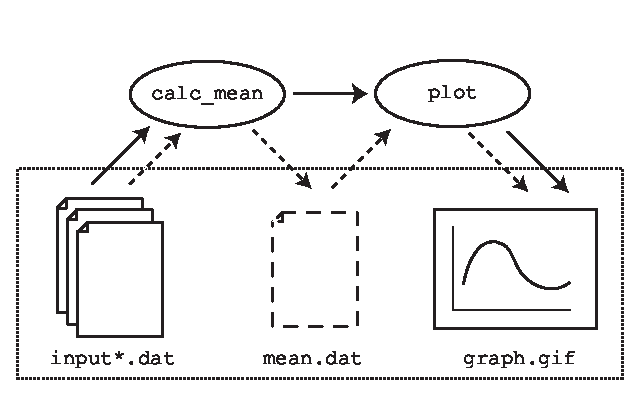
\includegraphics[height=4.2cm]{datapassing.eps}
\caption{NEED TO UPDATE THIS FIGURE. Illustration of direct data passing between VEIGA applications.  The ellipses are applications that are deployed on VEIGA servers and the dotted box represents the client's machine.  The dashed arrows represent data transfers that result from the first script in section~\ref{sec:workflows}.  The intermediate file {\tt out.dat} is not required by the client and so the workflow can be arranged so that this file is passed directly between the VEIGA servers (solid black arrows).}\label{fig:datapassing}
\end{figure*}

Data can also be streamed from one VEIGA application to the next through use of the pipe operator, for example:

\begin{verbatim}
myprog input.dat | plot > graph.gif
\end{verbatim}
See [REF] for more details.

Although very convenient, this method of constructing workflows using shell scripts has some weaknesses. The inputs and outputs of VEIGA applications (just like local applications) are files and so the ``workflow engine'' (i.e.\ the shell environment) performs no type checking on these entities.  The reponsibility of checking for validity of inputs is left to the applications themselves.  Secondly, although constructs such as loops are supported by the shell, the variables used to control these loops cannot be read directly from the outputs of the applications.

\section{Running multiple jobs with Condor}\label{sec:condor}
So far we have examined applications that run on the VEIGA server itself.  The simplicity and ease of use of VEIGA can be combined with the power of Condor to allow users to run applications multiple times over different inputs.  Condor [REF] is a popular and mature system for running applications in this manner.  Large numbers of machines (which are commonly ordinary desktop machines) can be brought together in a ``pool'' and users can execute their applications on this pool.  It is commonly employed in Monte Carlo simulations, parameter sweeps and other tasks that require ``high-throughput computing'' (HTC).  These tasks are extremely common in scientific computing.

A VEIGA server can be set up on a Condor submit host (i.e.\ a machine that is able to submit jobs to a particular Condor pool).  In this case, the applications that are deployed on the VEIGA server can be run on the Condor pool.  A single instance of an application can be run exactly as described above: there is no change from the user's point of view, except that interactive use will not be supported (section~\ref{sec:interactive}).  In this case, Condor is essentially being used for load balancing, ensuring that different instances of the application run on different hosts.

A very important and powerful new feature in VEIGA is the ability to run multiple jobs with a single command.  Let us imagine that the user wishes to run the  {\tt lbflow} application (section~\ref{sec:basicveiga}) over a hundred different input files, each containing a different configuration.  The user would place the input files in a local directory called ``inputs'' and run the following command from his or her local machine:

\begin{verbatim}
lbflow -i inputs -o outputs
\end{verbatim}
(Again, this assumes that the user has created a script called {\tt lbflow} that wraps the {\tt veigarun} program.)  The {\tt inputs} directory and its contents are uploaded to the VEIGA server as before.  VEIGA recognizes that the user has specified a directory of inputs instead of a single file and therefore it knows that it must run the {\tt lbflow} program many times, using a different input file each time.  This is achieved through Condor.

Each instance of the {\tt lbflow} program produces an output file and writes data to its standard output as before.  These output files are automatically downloaded by the VEIGA client software and are placed in the {\tt outputs} and {\tt stdout} directory respectively.  An information file is downloaded that tells the user which input files correspond to which output files, and also details whether each individual job was successful or not.

\section{Using VEIGA to submit jobs to Globus resources}
The Globus Toolkit (GT, [REF]) is a widely-used open-source toolkit for building Grid systems and applications.  It is now in version 4, although most production Grids (including the UK National Grid Service) are based on version 2.  The Globus Toolkit is a mature and feature-rich system but its complexity means that novice users find it difficult to use and the software itself can be difficult to install due, for example, to dependency issues.

Many projects [REFs] have dealt with this issue by hiding the complexity of Globus behind a more user-friendly interface and the same can be achieved with VEIGA.  SAY MORE HERE - MENTION CONDOR-G.

\section{Discussion}
We have presented VEIGA, a Very Easy Interface to Grid Applications. We have shown how applications can be deployed on a VEIGA server and run by users in exactly the manner in which they would run local programs.  The authors hope that the VEIGA system will greatly reduce the barrier to uptake of Grid technology by providing users with familiar interfaces to Grid resources.

The intutive VEIGA interface can be used to submit jobs to Condor pools and Globus resources.  In this respect there is clear overlap between VEIGA and other job submission and monitoring systems such as GridSAM.  There are advantages and disadvantages to both systems.  For example, GridSAM does not currently allow multiple job submission (section~\ref{sec:condor}) due to limitations in the Job Submission Description Language (JSDL) on which it is based.  However, GridSAM is currently more mature and robust than VEIGA and supports the execution of jobs on more back-end systems such as Sun GridEngine.  We are actively seeking collaboration with the GridSAM developers and intend to minimize the duplication of effort between the two systems.

The main areas in which VEIGA requires improvement are robustness and fault tolerance.  Improvements need to be made to ensure that the system responds gracefully to failures at both the server and client.

\section*{Acknowledgements}


\end{multicols}

\bibliographystyle{ametsoc}
\bibliography{refs}

\end{document}


